\documentclass{article}
\usepackage{amsmath,amssymb,complexity}
\usepackage{comment}
\usepackage{graphicx}
\usepackage{float}
\title{Project 2 : Crawling and Data Collection on the Web}
\author{Aashith Kamath Manjeshwar\footnote{Email : aashithk@cs.ucla.edu, UID : 504414409} 
\and Daksha Asrani\footnote{Email : dakshasrani@cs.ucla.edu, UID : 304432268}
\and Saikrishna Badrinarayanan\footnote{Email : saikrishna@cs.ucla.edu, UID : 904432289} 
\and Sayali Santosh Rajwade\footnote{Email : sayalirajwade@cs.ucla.edu, UID : 704406328}}

%\newcommand{\R}{\mathbf{R}}
%\newcommand{\U}{\mathbf{U}}
%\newcommand{\V}{\mathbf{V}}
%\newcommand{\W}{\mathbf{W}}

\usepackage{graphicx}
\graphicspath{ {plots/} }
\begin{document}
\maketitle

\paragraph{1)}

The hashtag we chose for this question is: $\#$brandbowl. The Topsy API was used to obtain the top five tweets. The 'limit' 
field in the code was set to '5'. The tweets are stored as a list in the object ret['response']['results']['list'].
The 'top\_tweets.txt' file contains each tweet item in the list in a single line.

The tweet text, user posting the tweet and the posting date of the top five tweets are as follows:

\begin{table}[H]
\centering
\begin{tabular}{ |p{.4cm}| p{6cm}| p{2.4cm} |p{2cm} |}
\hline
%\newline

\centering No. & \centering Text & \centering User & Posting Date \\ [0.5ex]

\hline
1 & \#brandbowl http://t.co/QoiFznuBKF & \centering darth & 1422837061 \\
2 & The new McDonald's positioning on \"I\"m loving YOU\" is a good messaging extension from I'm loving it \#brandbowl 
\#superbowlads & \centering jowyang & 1422837394\\
3 & \#GoDaddy goes small with a very tame, sweet ad \#BrandBowl & socialmedia2day & 1422837650 \\
4 & A Fiat just took some Viagra. Yep, that happened. \#SuperBowl \#BrandBowl & LinkedInQueen & 1422837660 \\
5 & Last chance to Retweet this for chance to win \$100 in \#SuperBowl swag. Join 
\#Jet \@ http://t.co/d1dsM3YSWR \#brandbowl http://t.co/8ulfL1UkPN & \centering DaveKerpen & 1422838470 \\
\hline
\end{tabular}
\end{table}

\paragraph{2)}
We use a script that, on a given hashtag, queries the topsy API repeatedly to get the entire set of tweets in the 
chosen time frame of one hour from 16:00 to 17:00 hrs PST on 2/1/2015. We repeat this process for all the 
five hashtags. However, the aforementioned API can only return a maximum of 500 tweets for any particular time frame. Thus, 
to get the entire set of tweets in a time frame, we solve the problem recursively (and dynamically). We first check the 
number of tweets for the entire time frame. If the number of tweets returned is 500, we recursively solve the problem 
for smaller segments of the time frame (half in this case) until the number of tweets returned by the API is lesser than 
500. This approach ensures that every single tweet in the time frame is collected even for extremely high rate of tweets 
at any instant. The results are stored in the file 'tweets.txt'. One issue that arises in this method is that we may have
duplicates in our file. This is because suppose a tweet had two of our hashtags in it. We would store that tweet on two 
occassions - once each when we are querying each of those two hashtags. So, we remove duplicate lines from the 'tweets.txt' file.
We also log information about the 
queries made as mentioned in the question in the file 'search\_log.txt'.
The hashtags with their tweet counts are as follows:
\begin{itemize}
 \item 
\#brandbowl - 4648
\item
\#SB49 - 92574
\item
\#football - 2084
\item
\#MakeSafeHappen - 2390
\item
\#adbowl - 0
\end{itemize}

%Thus, \#SB49 seems to be the most popular hashtag for the given time period.\\
Also, from the results we observe that our dynamic approach is highly efficient and does not use too many queries. For 
instance, the final hashtag \#adbowl has 0 tweets in the given period and this is solved in just 1 single query.
If we had split the timeframe into several slots, the smallest of which ensures that no hashtag has more than 500 tweets in
any such slot, then we would have to query the API several more times unnecessarily leading to the execution becoming much
slower.
 
\paragraph{3)}
In this question, we first compute a count of the number of tweets for each of the five hashtags in the time interval
from 16:00 to 17:00 hrs (PST) on 2/1/2015. This has essentially been calculated
in the previous question itself. Then, we plot a bargraph with the hashtags on the x-axis 
and the number of tweets on the y-axis. \\
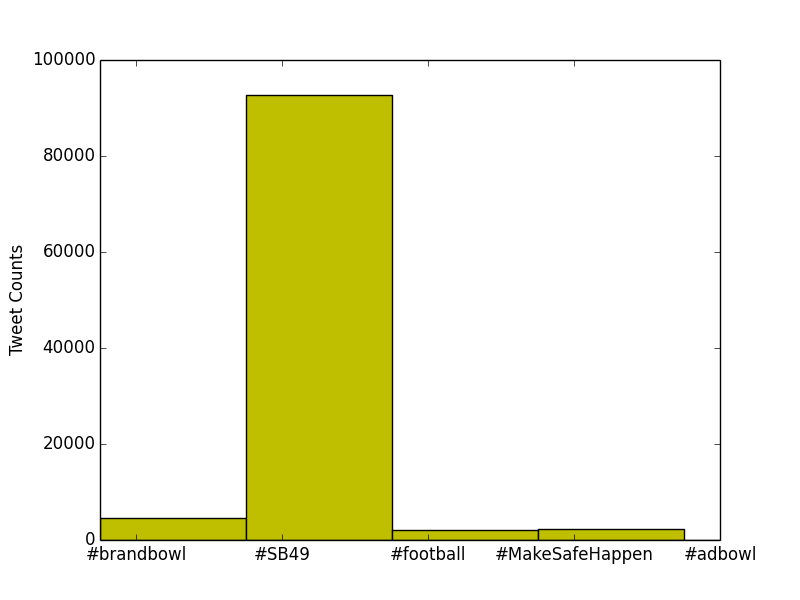
\includegraphics[scale=0.6]{Q3a_plot} 
The next part of the question involves calculating the number of tweets/second for different ranges of time (within that one hour)
for the most popular hashtag. From the results of the first part of the question, we observe that the most popular hashtag
is \#SB49. We choose a time interval of 3 seconds and query the API 1200 times (dividing one hour
into 1200 slots of 3 seconds each) obtaining the number of tweets in each of those slots. 
We then plot a graph with the start time of each slot on the x-axis and the number of tweets/second within that slot
on the y-axis. Actually, we plot two graphs - one has just the points alone while the other also contains a curve fit
between the points.
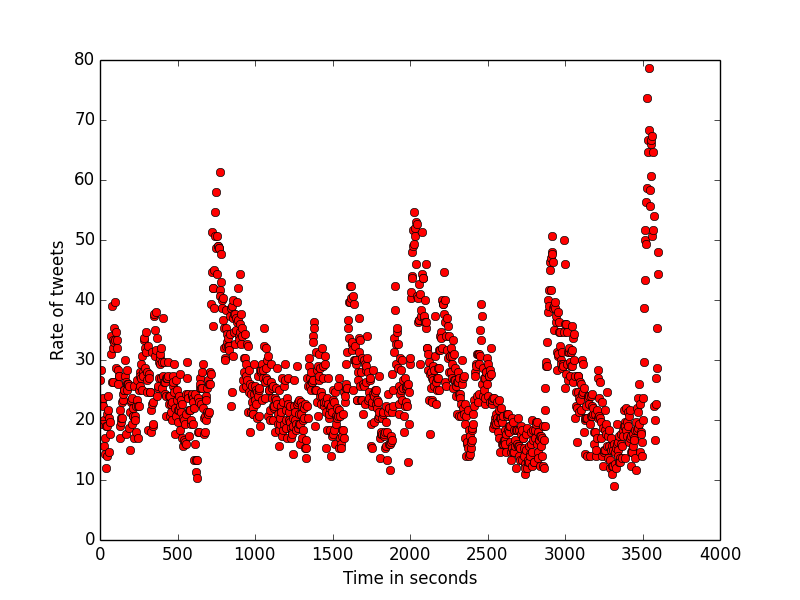
\includegraphics[scale=0.6]{Q3b_plot2} 
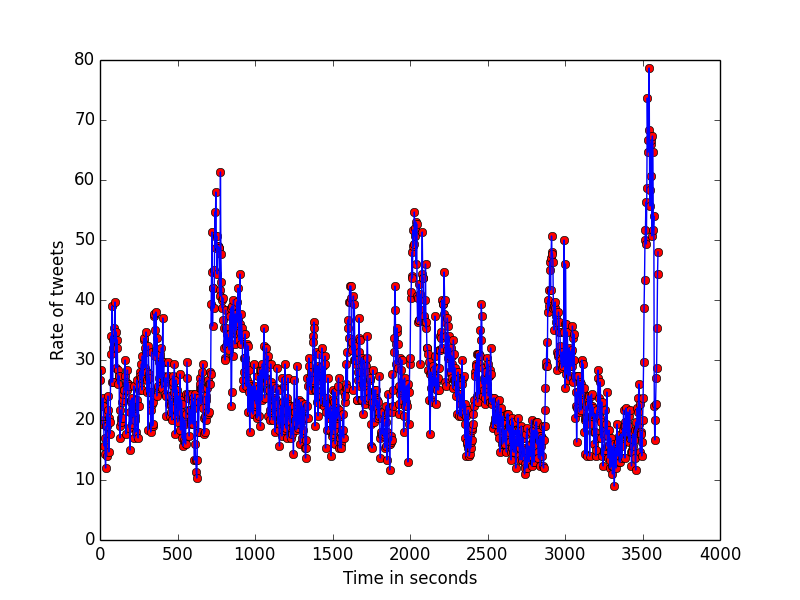
\includegraphics[scale=0.6]{Q3b_plot1} 

\paragraph{4)}
In this question, we compute the number of retweets for each tweet. First, we calculate the maximum number of retweets
for any tweet and this turns out to be 537. Then, for each $k \in \{1,2,\ldots,537\}$ we compute the number of 
tweets which have been retweeted $k$ times. We plot a graph with the x-axis containing the 
number of retweets $k$ (running from $1$ to $537$), and the y-axis containing the number of tweets retweeted $k$ times.
We use the polyfit function from the numpy library to see if we can fit a line to this plot.
The line is also displayed in the same figure along with the plot. The green line denotes the line we are
trying to fit and the blue line is the original plot.\\
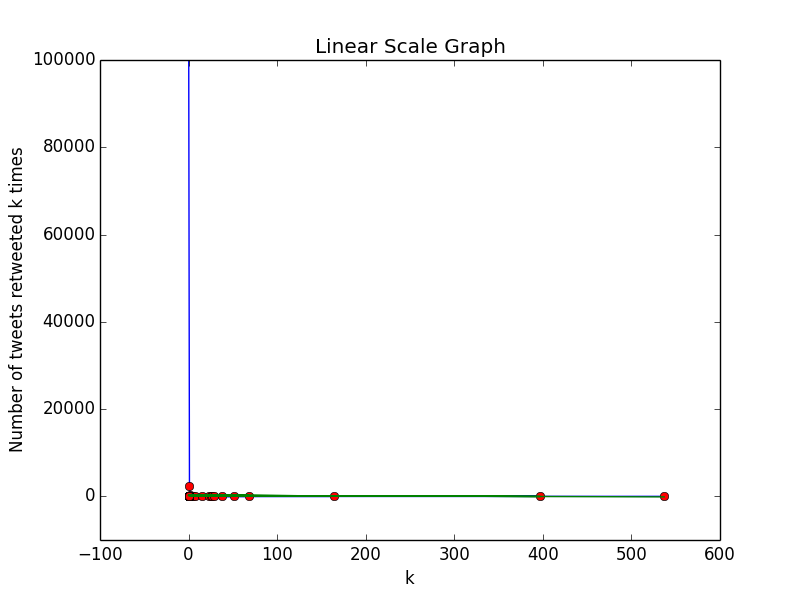
\includegraphics[scale=0.6]{4linear}\\ 

We then repeat the above plot on a log-log graph. We observe from the graph generated that we can't fit 
a line to this plot.\\
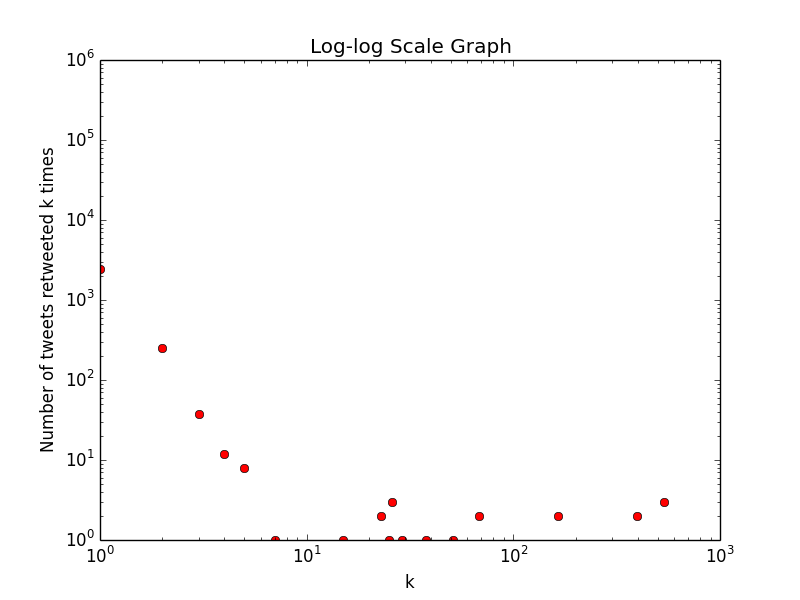
\includegraphics[scale=0.6]{4log} 
\paragraph{5)}
The two most popular hashtags are \#SB49 and \#brandbowl in that order.
We queried the API with a time interval of 3 seconds for the number of tweets containing each of those hashtags.
The timeframe was chosen as 3 seconds because after running question 2, we observed that for all the hashtags, there aren't 
500 or more tweets on any interval of 3 seconds or lesser.\\
We first plot a graph with the y-axis containing the number of tweets/second for \#SB49 and the x-axis
containing the start time for each slot.\\
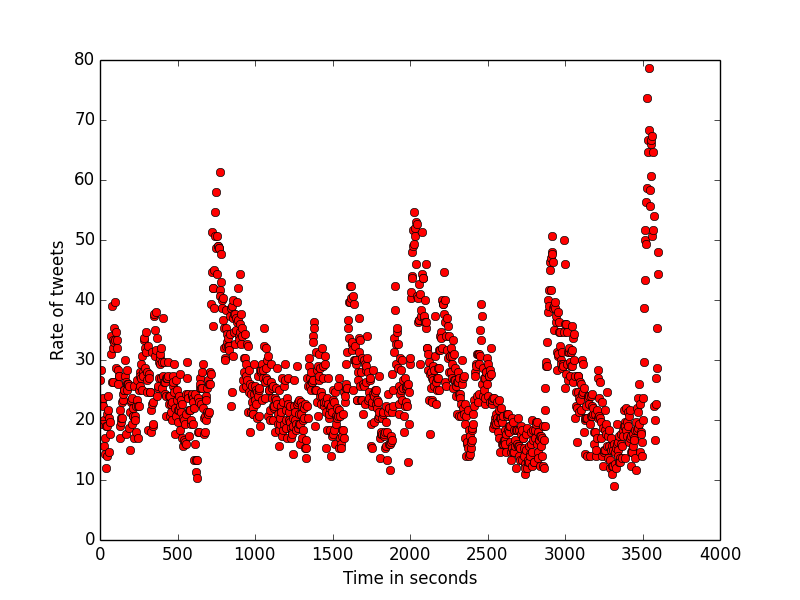
\includegraphics[scale=0.5]{Q3b_plot2} \\

The second plot has the number of tweets/second for \#brandbowl
in the y-axis and the start time of each slot in the x-axis.\\
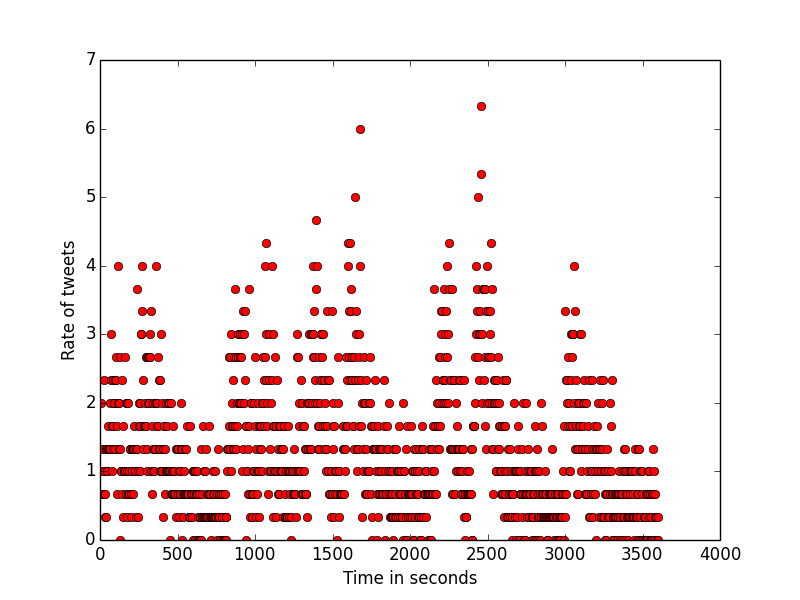
\includegraphics[scale=0.5]{5b}\\
We plot another graph
that has the number of tweets/second for \#SB49 on the x-axis and the number of tweets/second for \#brandbowl on the y-axis.\\

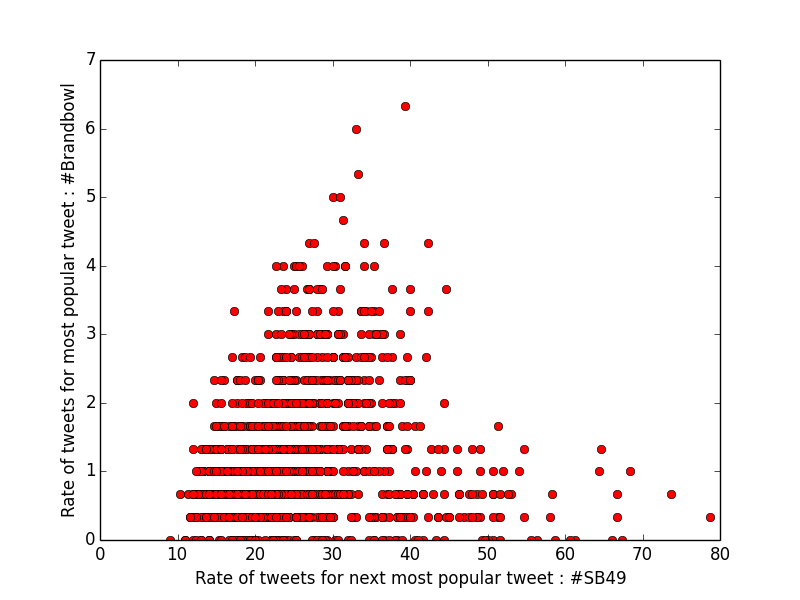
\includegraphics[scale=0.5]{5c}\\
There are 1200 points in 
each of these graphs since the overall time interval is an
hour and we have slots of 3 seconds each. 
We observe that these three graphs 
don't give us enough information to determine the correlation between the two hashtags. As a result, we construct 
a fourth graph to determine this information more clearly.\\

We choose time slots of 30 seconds each. For each time slot, we count the number of tweets in that slot for each
of the hashtags. We do this not by querying the API but by summing up the values we obtained earlier for the 3 second slots.
Querying the API again would be more time consuming and potentially inaccurate as the number of tweets in 30 seconds
could exceed 500 and the API would then return that as 500. After that, we cumulatively add the number of tweets. That is,
we count the number of tweets/second for the first 30 seconds in our timeframe, then for the first 60 seconds, then the first 90
and so on till we reach 1 hour. We plot a graph with the x-axis containing the number of tweets/second for \#SB49
and the y-axis contains the number of tweets/second for \#brandbowl. The plot has 120 points as there are 120
time slots of 30 seconds each in an hour. Our choice of 30 was not random. We tried a few different values 
ranging from 3 seconds to 1 minute and this seemed to give the most ``informative'' graph. The resulting graph
gives us a good indication of how closely the two hashtags are correlated.\\
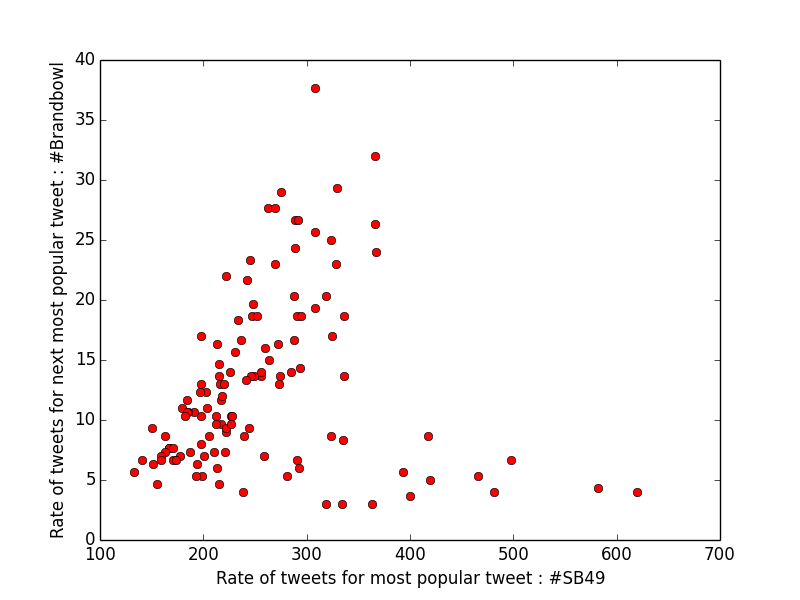
\includegraphics[scale=0.5]{5d}\\
\paragraph{6)}
Each line of the 'tweets.txt' file is parsed by using the json.loads() function. 
The tweet's post date, text, number of retweets, and the user posting it are printed out in the 'Output - Q6.txt' file
attached along with this report.
 \end{document}
